\documentclass[letterpaper,twocolumn,superscriptaddress,showkeys,longbibliography]{revtex4-1}
\usepackage[utf8]{inputenc}
\usepackage{color,dcolumn,graphicx,hyperref}
\hypersetup
{
    colorlinks = true, linkcolor = blue, citecolor = blue, urlcolor = blue,
}

\begin{document}

\title{Developing a preprint culture in biology}

\author{Philippe Desjardins-Proulx}
\email[E-mail: ]{philippe.d.proulx@gmail.com}
\affiliation{Theoretical Ecosystem Ecology laboratory, Universit\'e du Qu\'ebec \`a Rimouski, Canada.}
\affiliation{Quebec Center for Biodiversity Science, McGill University, Canada.}

\author{Ethan P. White}
\affiliation{Departement of Bology, Utah State University, United-States of America.}

\author{Joel J. Adamson}
\affiliation{Ecology, Evolution and Organismic Biology, University of North
Carolina at Chapel Hill, United-States of America}

\author{Timoth\'ee Poisot}
\affiliation{Theoretical Ecosystem Ecology laboratory, Universit\'e du Qu\'ebec \`a Rimouski, Canada.}
\affiliation{Quebec Center for Biodiversity Science, McGill University, Canada.}
\affiliation{International Network for Next-Generation Ecology.}

\author{Karthik Ram}
\affiliation{Environmental Science, Policy, and Management. University of California, Berkeley, United-States of America.}

\author{Dominique Gravel}
\affiliation{Theoretical Ecosystem Ecology laboratory, Universit\'e du Qu\'ebec \`a Rimouski, Canada.}
\affiliation{Quebec Center for Biodiversity Science, McGill University, Canada.}

\keywords{Publishing; Preprint servers; Green Open Access; arXiv.}

\maketitle

\section{Introduction}

Public preprint servers allow authors to make manuscripts publicly available
before, or in parallel to, submitting them to journals for traditional
peer-review. The rationale for preprint servers is fundamentally simple: to make
the results available to the scientific community as soon as possible rather
than to wait until the peer-review process is fully completed. The goal of arXiv
and open preprint servers is not to circumvent the peer-review process; almost all
manuscripts on arXiv are submitted to peer-review.  Sharing ideas as quickly as
possible using preprint servers has numerous advantages.  These include rapid
dissemination of work-in-progress to a wider audience, including readers in
developing countries where access to subscription journals is often a limiting
factor in scientific research.  Furthermore, preprints provide the opportunity
to solicit feedback from a larger pool of reviewers and can be seen as an
integral aspect of a vigorous peer-review process \cite{hoc12}.  Preprint
servers therefore increase the number of opportunities for review and revision
prior to publication, resulting in higher quality submissions and also could
alleviate reviewer burden.

Preprints gained popularity 20 years ago with the advent of arXiv, an open
preprint server widely used in physics and mathematics \cite{nie08,gin11}. Preprints
are also integral to the culture of other scientific fields.  Paul Krugman noted
that, in economics, the \emph{traditional model of submit, get refereed,
publish, and then people will read your work broke down a long time ago. In
fact, it had more or less fallen apart by the early 80s} \cite{kru12}. In
addition to a section in arXiv, economists have also the RePEc (Research Papers
in Economics) initiative, which aims to create an archive of working papers,
manuscripts, and book chapters.  Despite the success of this approach in other
fields, most manuscripts in biology are not submitted to a public archive before
being submitted to peer-review. In this article, we first highlight the
advantages of open preprint servers for both scientists and publishers. We
then debunk a few misconceptions, discuss the policies of major publishers in
biology, and briefly review the most popular open preprint servers currently available.

\section{The case for public preprints}

The first and most often discussed advantage of arXiv and open preprints is
speed (Figure~\ref{fig:map}). The time between submission and the official
publication of a manuscript can be measured in months, sometime in years. For
all this time, the research is known only to a select few: colleagues, editors,
reviewers. Thus, the science cannot be used, discussed, or reviewed by the wider
scientific community. In a recent blog post, C Titus Brown noted how posting a
paper on preprint lead to a quick citation (arXiv papers can be cited) and his
research was integrated by another researcher \cite{bro12}. The current system
of hiding manuscripts before acceptance pose problems for both scientists and
publishers. Manuscripts that are unknown cannot be used and thus take more time
to be cited. It has been shown that high-energy physics, with its high arXiv
submission rate, had the highest immediacy among physics and mathematics
\cite{pra05}. Immediacy measures how quickly articles are cited. 

Furthermore, the review process as a whole is critically over-loaded, because
the number of active scientists increases, because the pressure to publish
increases, and because of an effect dubbed ``the tragedy of the reviewers
commons'' \cite{hoc09}.  At the same time, rejection rates are high in most journals
\cite{aar08,roh09}, and when not invited to submit a revision, authors must start the whole
process all over again.  Initiatives to reduce time from submission to
publication have emerged across the scientific community. Rohr et al.
\cite{roh09} called for the recycling and reuse of peer-reviews:
by attaching previous reviews and detailed replies to a new submission, both
the editor and the referees can gauge the work done on the manuscript, and
perhaps evaluate it with less prejudice. In a similar way, the \emph{Peerage
of Science} initiative allows authors to seek anonymous pre-review by their
peers. Some journals now accept to publish papers which received good
evaluations, with \emph{Animal Biology} having recently accepted first a paper
reviewed entirely with the \emph{Peerage of Science} \cite{abb12}, effectively
outsourcing the review process. A widespread use of preprint servers can
achieve the same goal of reducing the time spent in review. By putting a
manuscript for open comments and criticisms, the authors will receive valuable
feedback and can improve the version which will be submitted. With a rich
enough community of scientists depositing preprints, and commenting on them,
the process of an open pre- review can become widespread and will overall
increase the quality of first submissions.

\begin{figure}[ht!] \centering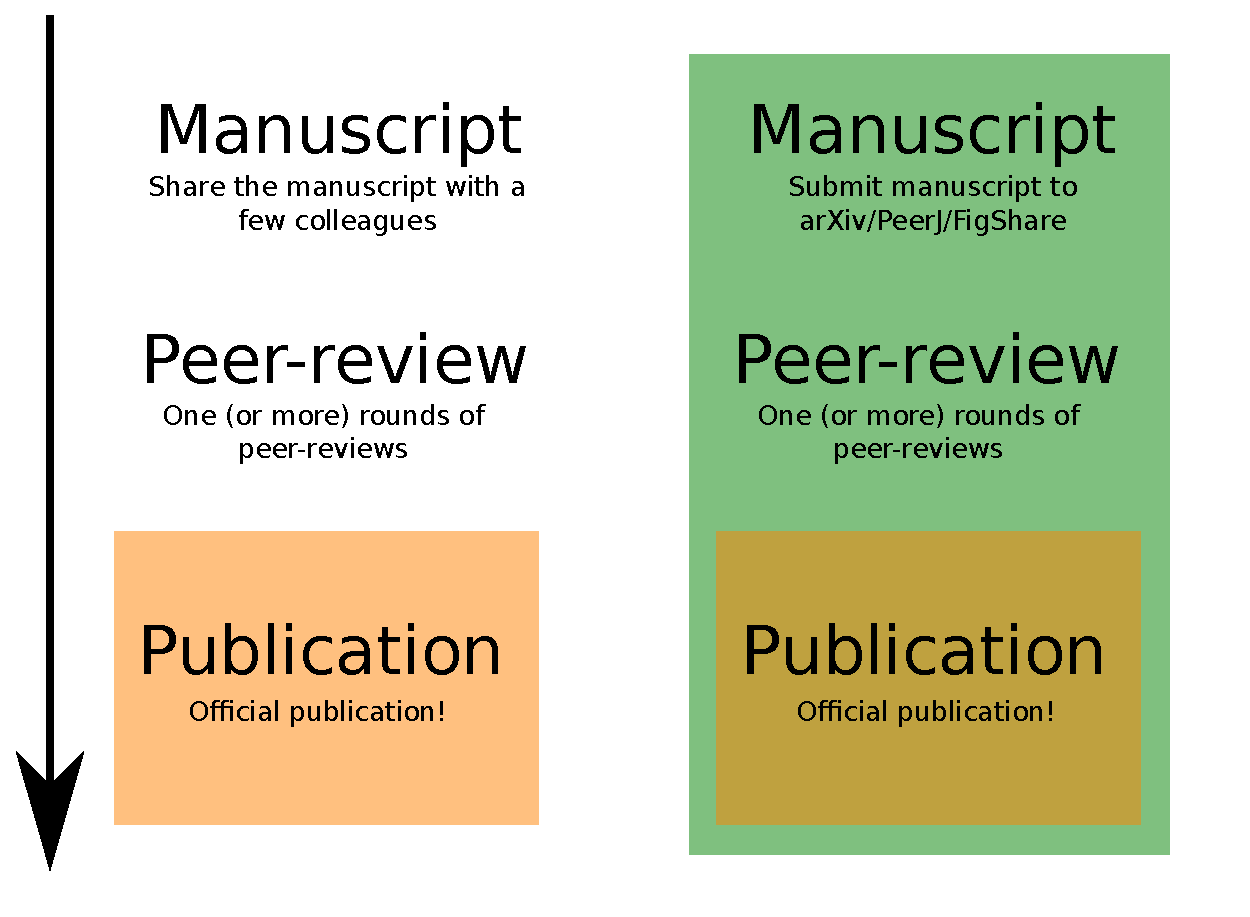
\includegraphics[width=0.50\textwidth]{map.pdf}
\caption { It can take several months, and even a few years, before a submitted
paper is officially published and citable.  The average time to publication
varies greatly between journals and can be as low as 104 days (Evolution for
2011) to 213 (PLOS One in 2010).  Meanwhile, few people are aware of the
research that has been done since, typically, only close colleagues are given
access to the preprints. With public preprint servers, the science is
immediately available and can be openly discussed, analyzed, and integrated into
current research. It benefits both science and publishers. Both want the papers
to be well-known and cited, and public preprints make it possible to integrate
research even before publication, greatly improving immediacy.  }
\label{fig:map} \end{figure}
% Dom : Do you have a reference for the stats in the legend?

Public preprint servers offer a much fairer way to establish intellectual
priority by making the work available when done. Some manuscripts will spend
much more time in the review process than others. Surprisingly, there is a
perception in biology that public preprints make it easier to steal ideas, as if
a scientific idea was only complete once published in a peer-reviewed journal
\cite{gin11}. Ironically, mathematicians and physicists have embraced arXiv in
part to establish priority in a fair way \cite{gin11,cal12}.
% Dom: That's a very interesting statement, if not the best one to justify preprints. Could you develop just a bit more the argument?

Prepublication reviews by a small network of colleagues is an important part of
the scientific process, attested by the fact that nearly all published papers
acknowledge comments by people not listed as co-authors.  Preprint servers
simply offer a way to extend this network of colleagues to the entire scientific
community. It ensures that science is not constrained by small networks of
scientists exchanging ideas.  Paul Ginsparg created arXiv.org in part for
democratic reasons: he wanted everyone from students in small universities to
Ivy-League professors to have access to the most recent scientific \emph{ideas}.
Ginsparg's revolutionary idea was simply to use the power of the internet for
preprints, not just for the end product, so the scientific process can be open
as soon as possible.
% Dom: I do accept this argument, although I have doubts it makes any difference. Just think about the number of comments posted on PLoS One...

\section{Preprints in biological sciences}

Submitting to a preprint server is becoming more common in biology, even though
it still involves a minority of papers. The quantitative biology section in
arXiv is experiencing faster growth in submissions than any other field
\cite{cal12}. Most scientific journals are preprint-friendly: Nature, PLOS, BMC,
PNAS, Science (mostly) \ref{table:policies}, and all the journals from Elsevier %something is off in the formatting here
and Springer.  The Ecological Society of America and the Genetics Society of
America recently changed their policies to allow public preprints.  Few
scientific publications will not consider a manuscript submitted to a public
preprint server.  Still, a few journals adopt a ``by default'' hostile attitude
towards preprints, mostly due to the lack of clear policy of the publishers, or
perhaps because a preprint culture has not developed in biology and the practice
is still considered unusual. As an example, Wiley-Blackwell, which publishes
some leading journals, has no official policy on the subject
\ref{table:policies}.

Part of the hostility to preprints servers comes from a certain interpretation
of the Ingelfinger rule: scientists should not publish the same manuscript twice
\cite{alt96}. However, papers submitted to arXiv or other preprints servers are
only published in one peer-reviewed journal. A preprint is just a preprint, it
is a document that allows ideas to spread and be discussed, but it is not yet
formally validated by the peer-review system, which is why the majority of
publishers does not see arXiv and similar services as a violation of the
Ingelfinger rule. \emph{Nature} responded to the rumour that they refused
manuscripts submitted to arXiv by saying that ``\emph{Nature} never wishes to
stand in the way of communication between researchers. We seek rather to add
value for authors and the community at large in our peer review, selection and
editing'' \cite{nat05}.

\begin{table*}
    \centering
    \begin{tabular}{|ll|}
    \hline
    Publisher                                   & Policy \\
    \hline
    Springer                            	& Accept \\
    BMC                                 	& Accept \\
    Elsevier                            	& Accept \\
    Nature Publishing Group             	& Accept \\
    Public Library of Science           	& Accept \\
    Genetics Society of America                 & Accept \\
    Royal Society                       	& Accept \\
    National Academy of Science (USA)           & Accept \\
    Ecological Society of America       	& Accept \\
    Oxford Journals                             & Accept \\
    Science                             	& Ambiguous \\
    Wiley-Blackwell                       	& No general policy \\
    British Ecological Society                  & No answer to our query \\
    \hline
    \end{tabular}
    \caption{Policies for important publishers in biology. Some publishers
tolerate preprints except for a few of their medical journals, e.g.: Journal
of the National Cancer Institute from Oxford and The Lancer from Elsevier.}
    \label{table:policies}
\end{table*}

\section{Current offerings}

We briefly discuss the main options to submit preprints to open servers:
arXiv.org, figshare, and the upcoming PeerJ and F1000Research.

\subsection{arXiv}

arXiv (\url{http://arxiv.org/}) is the most widely-used preprint server today,
and its use is almost universal in some branches of mathematics and physics.
arXiv provides a reliable citation system for all eprints and is especially
popular in high-energy physics. Physicist Paul Ginsparg created arXiv in 1991
for theoretical high-energy physicists to communicate preprints via email and
ftp, and soon thereafter adopted the newly created world-wide
web\cite{jackson2002preprints}.  arXiv now receives over 7 000 submissions per
month (\url{http://arxiv.org/show_monthly_submissions}) and divides its
submissions into subcategories of physics, mathematics, computer science,
quantitative biology, finance and statistics.  The quantitative biology category
includes subcategories for Populations and Evolution, Quantitative Methods and
other categories that may be of interest to biologists.

Submission to arXiv is fully automated.  Authors can submit \TeX{}/\LaTeX{}
documents that are compiled on the server or directly submit in PDF/PS format
(for example, as exported by a word processor).  A moderation system was put in
place in 2004: papers must be categorized by an endorser. At least one author of
a paper must be an endorser that has previously submitted a paper or has
received permission to submit to a particular category.  Many authors in
mathematics and physics submit papers as soon as they are ready for review by
colleagues, although another popular option is submitting simultaneously to a
journal and arXiv.

Authors must either have their arXiv submission available under an open license
or grant arXiv a non-exclusive and irrevocable license to distribute the work.
In either case, arXiv does not require copyright transfer and only requires the
rights to distribute submitted articles in perpetuity. Thus, submitting to arXiv
does not in itself prevent the authors from transferring their rights to a
publisher, which is why most publishers tolerate arXiv, even though they ask the
authors to transfer their right to them upon acceptance of the article.

Most papers posted to arXiv are eventually printed in journals but there are
notable exceptions, such as Perelman's landmark paper leading to the proof of
the Poincar\'{e} conjecture \cite{2002math.....11159P}.  However, arXiv has
never sought to replace scientific journals and explicitly states that it serves
a different function as ``an openly accessible, moderated repository for
scholarly articles in specific scientific disciplines.'' arXiv is now
administered by the Cornell University Libraries, with funding coming from
voluntary pledges by academic institutions along with matching funds from the
Simons Foundation \cite{arxiv_future}.  One-hundred twenty six of the top
two-hundred institutions in terms of downloads have provided the operating
budget for arXiv over the next five years.  This plan reduces the financial
burden on Cornell University and transfers governance to a collaborative
community in accordance with arXiv's key principles.  arXiv takes numerous
measures to ensure that the repository will remain permanently available and
submissions will be readable.

\subsection{figshare}

figshare (\href{http://figshare.com}{http://figshare.com}) is an open server
that allows scientists to submit any research output: manuscript, figures,
datasets, videos, theses, presentations, and so on. There are no rules to limit
what constitutes a research output and, unlike arXiv, there is no endorser
system. All figshare content has a unique digital object identifier (DOI) like
any journal article, thus offering a permanent and stable link to the content.
A flexible tag system is used to classify each item. All content can be
commented and is licensed under the Creative Commons (CC-BY) license, except
datasets which are published under CC0. The CC-BY license grants rights to
\emph{copy, distribute, display and perform the work and make derivative works
based on it only if they give the author or licensor the credits in the manner
specified by these.}  CC0 is the most permissive license and effectively puts
the work in public domain (no rights reserved) or, if it is not possible in the
given jurisdiction, provides a simple permissive license.

One of the biggest advantage of figshare over arXiv is that is it not limited to
quantitative sciences. arXiv.org has sections on quantitative biology but might
not be appropriate for non-quantitative work. With its flexible approach to
preprints, figshare offers an important alternative to arXiv for empirical
biologists. Furthermore, by allowing all types of content, figshare arguably
provides an archive for early results (e.g.: figures, lab presentations).

\subsection{PeerJ}

PeerJ (\href{https://peerj.com/}{https://peerj.com/}) is a new publishing system
that combines both a preprint server, and a peer reviewed journal.  It is
focused on the biological and medical sciences, which may help overcome the
perception that preprints do not have a home in biology.  PeerJ allows
commenting on posted preprints, improving the potential for pre-publication
dialog. In addition, preprints can be made private if the authors choose, and
shared only with selected colleagues. While this reduces some of the benefits of
preprints described above, it may allow some researchers who would not otherwise
post preprints to begin to explore the possibility in a manner appropriate to
their current circumstances.

In contrast to other preprint servers users cannot post unlimited public
preprints for free. One preprint per year can be posted for free and a onetime
(i.e. lifetime) fee of 99 dollars allows the posting of unlimited public
preprints. It is also worth noting that the preprint server is not tied to the
journal, so preprints can be posted regardless of where they will eventually be
submitted for publication.

PeerJ uses the CC-BY-SA 3.0 license, which is similar to the CC-BY license used
by figshare but adds the \emph{Share-alike} (sa) restriction that derivate works
need a license identical to the license that governs the original work.

\subsection{F1000Research}

F1000Research is not a public preprint server like the previous three servers.
Whereas arXiv, figshare, and PeerJ offer an option to submit a manuscript
without having it reviewed, papers submitted to F1000Research will eventually be
reviewed. Thus, F1000Research offers a hybrid model with publicly available
manuscripts at time of submission and standard peer-reviews. Manuscripts are
considered ``accepted'' and will only be indexed after two positive referee
response. F1000Research works closely with data providers to integrate raw data
to the paper. For instance, upon submitting a paper, authors are asked to upload
their data, which are then integrated in \emph{e.g.} figshare widgets, the DOI
of which are given in the paper when the data are first mentionned.  The
licensing of the data is similar to the one used by figshare, meaning that the
articles are free to access, and can be redistributed readily. By putting much
effort in integrating data to the paper, F1000Research is working to make
science more reproducible and open.

\subsection{GitHub}

This manuscript was developed entirely as an open project on GitHub. GitHub is
one of several hosting services for collaborative development using the Git
version control system (VCS).  Git is a decentralized revision control system
created by Linus Torvalds and is used primarily to develop software, including
the Linux kernel. Git provides powerful features that allow numerous
contributers to work asynchronously on the same project, often in parallel
branches, all of which can be effortlessly merged and version controlled.  While
Git is created primarily for software development, where the use of version
control systems is standard \cite{aru12}, it is ideal for academic research
since it provides a way to collaborate on every step of the manuscript
development process, from data manipulation and analysis to writing and
revision. For example, during the development of this manuscript, each author
would clone the project (\emph{i.e.} make a personal copy), modify it, and then
merge their changes into a master branch. This takes the preprint process to an
entirely new level, where the entire writing process is open from the beginning.

\section{Conclusion}

% Dominique:
% I added the following three paragraphs to the conclusion, offering also a
% discussion on the on going explosion of different publication models. Take
% what you want and remove what you don't need.  I also had the feeling we might
% want to include a single paragraph, very short, calling that evaluations
% (academia, grant agencies etc...) looking at publication records or report of
% scientific activities start to view preprints as a significant and sound
% scientific contribution. One of the most important benefit is again the speed
% of the publication process. Most grants are for three years or less. It makes
% it hard to have a published paper within the limits of the grant. Preprints
% could however speed the process and show that contributions were made during
% the time of the grant. 

The ongoing discussions on the publication process, peer-reviewing and
alternative publication models are all symptoms of the current uneasiness of
scientists with the ever growing obsession with bibliographic metrics such as
the impact factor \cite{Fisher2012}. There is pressure on researchers, wether
they are junior looking for an academic position or senior trying to secure
funding for their team, to orient their publication strategy in order to
maximize their number of publications and total citations. A well-known
consequence is to submit manuscripts first to the most prestigious journals, and
then resubmit to lower level journals as they are rejected. The numerous
negative impacts of such behavior have been discussed in depth \cite{hoc09} and
include a long delay between the time a manuscript is finished to its
publication.  They all contribute somehow in a general slowing down of
scientific progress.  Research activities and the publication process are
drifting away from their fundamental object, namely the diffusion of novel
scientific discoveries. 

Developing a preprint culture in biology is not a final solution to the impact
factor inflation, it might however reduce significantly its negative
consequences. Preprints speed up publication, openly, with no judgement on
pertinence and originality. Paradoxically, because peer-reviewing is conducted
following this step in the process of a scientific communication, it might bring
it closer to its fundamental objective. The role of peer-reviewing is to judge
the scientific quality of a study, the match between its hypotheses, methods,
results and conclusions. The peer review process is the first barrier against
fraudulent or bad quality science, susceptible to impede scientific progress. It
is however now dominated by subjective evaluations, where trendy contributions
are promoted to increase the immediacy impact of the journal. Most journals have
in their instructions for reviewers a section devoted to the evaluation of
suitability for the journal, a task usually incumbent to editors. Preprints are
by definition not evaluated, neither for their quality nor their pertinence.
Technically, the difference between a preprint and a traditional publication
should be that the latter as the approval stamp by pairs on its quality. The
relevance of a study, its contribution to science, should only be judged
post-publication by many more readers than the typical two-four anonymous
reviewers. With a such a shift in the diffusion strategy, the role of
traditional journals and their editors would be to showcase scientific
discoveries for specialized readership. Such a process should improve even
further their diffusion, not impede it. 

The current opening of the publication process we are currently witnessing with
the arrival of new preprint systems and innovative publication models such as
F1000, PLOS One, Nature Scientific Reports, might significantly bypass the
inflation of bibliographic metrics. They not only promote scientific communications
by changing the focus of peer-reviewing, they also favor the publication of
results that might otherwise be rejected because of low interest, negative
results, descriptive and quantitative studies and datasets. One of drawback of
making publication easier is obviously the proliferation of studies of uneven
quality. A tradeoff between the intensity of the peer-review filtering and the
benefits to science has been hypothesized \cite{Aarssen2012}. With increasingly
stringent peer reviewing, the quality of published papers and easiness of
finding discoveries might increase, at the cost of censorship, increasing load
on authors and reviewers and time for publication. Preprints are simply
bypassing this model, for what we believe is the progress of science: they speed
up the dissemination of scientific discoveries, impede censorship and put on
reader's shoulders the responsibility to judge originality and pertinence.

Open preprint servers offer a great opportunity for open science, especially if
the community embraces the idea of discussing preprints. Initiatives like
Haldane's Sieve (\href{http://haldanessieve.org/}{http://haldanessieve.org/}), a
new blog discussing arXiv papers in population genetics, will help make arXiv
attractive for scientists looking to promote their work. These initiatives are
important to fully exploit the potential of open preprints servers. Posting
preprints online increases the community of available informal peer reviewers,
and uses the internet for its original community-building purposes.

% Aren't we bridging more than cultural and geographic? I mean, we are
% essentially cross pollinating ideas. e.g. It took a lot time for MCMC to
% become popular in ecology even though it was widely used in other disciplines
% a decade or two earlier.
Preprint servers also facilitate communication between disciplines, bridging
cultural as well as geographic divides. Examples include a recent series of
papers on the theory of natural selection that was posted to arXiv
simultaneously with its publication in the \emph{Journal of Evolutionary
Biology} \cite{JEB:JEB2431,JEB:JEB2498,JEB:JEB2378,JEB:JEB2373}. Other
submissions in this category include evolutionary and ecological theory by
authors trained in physics and computer science.  Since authors in these fields
regularly check arXiv, submitting preprints may be the most effective way
biologists can help others avoid ``repeated work'' \cite{de2011contribution} and
form a synthetic community of evolutionary theorists from disparate backgrounds.
The advantages are clear and the costs are low.

\section{Funding}

PDP is supported by an Alexander Graham Bell scholarship from the National
Sciences and Engineering Council of Canada. EPW is supported by a CAREER Award
from the National Science Foundation (DEB-0953694). JJA is supported by NSF
DEB-0614166 and NSF DEB-0919018. KR is supported by NSF DEB-1021553. DG is
funded by a Discovery Grand from the National Sciences and Engineering Council
of Canada and by the Canada Research Chair program.

\section{Acknowledgements}

We thank Carl Boettiger and Mark Hahnel for helpful comments on an earlier
version of this manuscript.

\newpage
\bibliography{refs}

\end{document}

